\documentclass[11pt,a4paper]{article}
\usepackage[T1]{fontenc}
\usepackage[utf8]{inputenc}
\usepackage[polish]{babel}
\usepackage[margin=2.3cm]{geometry}
\usepackage{lmodern,microtype}
\DisableLigatures{encoding = T1, family = lmtt}
\usepackage{array,longtable,booktabs,tabularx}
\usepackage{amsmath,amssymb}
\usepackage{graphicx,xcolor,tikz,listings}
\usetikzlibrary{arrows.meta,positioning,fit,backgrounds,shapes.geometric,shapes.multipart}
\usepackage[hidelinks,unicode]{hyperref}
\usepackage{xurl}
\usepackage{bookmark}
\usepackage{enumitem}
\usepackage{placeins}
\graphicspath{{pz/lab3/}{./}}

\definecolor{accent}{HTML}{245777}
\definecolor{pale}{HTML}{EDF3F7}
\definecolor{codebg}{HTML}{F5F5F5}
\hypersetup{
  pdftitle={TSDB -- implementacja rdzenia systemu i raport z postępów},
  pdfauthor={Hubert Błonowski, Jan Zaborski}
}
\setlength{\emergencystretch}{2em}
\setlength{\parskip}{0.35em}
\setlength{\parindent}{0pt}
\setcounter{tocdepth}{1}
\setlist{itemsep=0.15em,topsep=0.3em}
\renewcommand{\arraystretch}{1.18}
\setlength{\tabcolsep}{2.8pt}
\newcolumntype{P}[1]{>{\raggedright\arraybackslash}p{#1}}
\newcolumntype{Y}{>{\raggedright\arraybackslash}X}
\newcommand{\code}[1]{\expandafter\nolinkurl\expandafter{\detokenize{#1}}}
\newcommand{\tabhead}[1]{\toprule #1\\ \midrule\endfirsthead
  \toprule #1\\ \midrule\endhead \bottomrule\endfoot}
\lstset{
  basicstyle=\ttfamily\footnotesize,
  backgroundcolor=\color{codebg},
  frame=single,rulecolor=\color{black!15},
  breaklines=true,columns=fullflexible,keepspaces=true,
  showstringspaces=false,tabsize=2,
  aboveskip=0.8em,belowskip=0.8em
}
\tikzset{
  box/.style={draw=accent,rounded corners=2pt,fill=pale,
    align=center,font=\small,minimum height=11mm,text width=36mm},
  external/.style={box,fill=white,draw=black!60},
  arrow/.style={-{Latex[length=2mm]},thick,draw=accent},
  note/.style={font=\scriptsize,align=center,fill=white,inner sep=2pt},
  state/.style={box,text width=28mm,minimum height=10mm},
  umlclass/.style={draw=accent,fill=pale,rectangle split,
    rectangle split parts=3,rectangle split part align={left,left,left},
    align=left,font=\scriptsize,
    inner sep=5pt,text width=43mm},
  assoc/.style={thick,draw=accent},
  compose/.style={{Diamond[fill=accent,length=2mm]}-,thick,draw=accent},
  usecase/.style={ellipse,draw=accent,fill=pale,align=center,
    font=\small,text width=36mm,minimum height=13mm}
}


\begin{document}
\raggedbottom
\hypersetup{pageanchor=false}
\begin{titlepage}
	\centering
	{\large Politechnika Warszawska\\
		Wydział Matematyki i Nauk Informacyjnych\par}
	\vspace{2.1cm}
	{\Large Projekt zespołowy -- laboratorium 3\par}
	\vspace{1.2cm}
	{\huge\bfseries Implementacja bazy danych\\
		szeregów czasowych\\w języku Rust\par}
	\vspace{1.1cm}
	{\LARGE Implementacja rdzenia systemu\\
		i raport z postępów\par}
	\vspace{1.4cm}
	\begin{tabular}{rl}
		Autorzy:          & Hubert Błonowski       \\ & Jan Zaborski\\[.5em]
		Promotor:         & mgr inż. Paweł Sobótka \\[.5em]
		Wersja dokumentu: & 1.0                    \\
		Data:             & 18 listopada 2026 r.
	\end{tabular}
	\vfill
	\url{https://github.com/janzaborski/rust-tsdb}
	\vspace{.8cm}
\end{titlepage}
\hypersetup{pageanchor=true}

\pagenumbering{arabic}

\section*{Opis projektu}
Projekt polega na stworzeniu jednowęzłowej bazy danych szeregów czasowych
w języku Rust. System gromadzi pomiary opisane czasem, wartością i etykietami,
przechowuje ich historię oraz udostępnia ją przez interfejs HTTP oraz ograniczony
podzbiór języka zapytań PromQL. Dodatkowo projekt uwzględnia
integracje interfejsu graficznego Grafana.

\section{Stan implementacji}
\begin{itemize}
	\item \textbf{Model danych i indeksowanie.}
	      Próbka zawiera znacznik czasu w milisekundach oraz wartość liczbową.
	      Zestaw etykiet identyfikuje szereg, a indeks odwrócony pozwala wyszukiwać
	      szeregi według nazw i wartości etykiet. Ten sam model obsługuje zapis i zapytania.

	\item \textbf{Bufor i segmenty dyskowe.}
	      Nowe pomiary trafiają do pamięci, i okresowo są
	      zapisywane w segmentach na dysku. Odczyt łączy historię z dysku z najnowszymi próbkami
	      w buforze. Sumy kontrolne wykrywają uszkodzenia segmentów, a blokada katalogu
	      uniemożliwia równoczesne otwarcie tej samej bazy przez dwa procesy.

	\item \textbf{Dziennik WAL i odzyskiwanie.}
	      Dziennik rejestruje definicje szeregów i próbki przed aktualizacją bufora.
	      Przy starcie baza odczytuje segmenty i odtwarza pozostały WAL, uwzględniając
	      niepełny koniec dziennika. Po zrzucie danych usuwa zbędne zamknięte segmenty WAL.

	\item \textbf{Interfejs HTTP.}
	      Udostępnia odczyt diagnostyczny, zapytania chwilowe
	      i zakresowe, sprawdzanie gotowości oraz informacje o wersji.

	\item \textbf{Parser i wykonawca zapytań.}
	      Obsługiwane są nazwane selektory i dokładne dopasowanie etykiet.
	      Parser sprawdza składnię, a wykonawca wybiera próbki dla pojedynczej chwili
	      lub siatki czasu. funkcje agregujące pozostają do implementacji.

	\item \textbf{Integracja i demonstracja.}
	      Docker Compose uruchamia bazę i Grafanę, automatycznie konfigurując źródło
	      danych oraz dashboard. Przykładowy skrypt pobiera rzeczywistą telemetrie
	      systemu Windows i wysyła je co sekundę. Wolumeny zachowują historię
	      pomiarów po ponownym uruchomieniu kontenerów. System jest odporny na restart
	      poszczególnych procesów.
\end{itemize}

\clearpage
\section{Działanie rdzenia na przykładzie monitorowania CPU}
Poniższy opis przedstawia działanie systemu na dzień 18.11. Niektóre
szczegóły implementacyjne mogą ulec zmianie w kolejnych etapach projektu.

Załóżmy, że kolektor monitoruje obciążenie procesora komputera
\code{pc-demo}. Poniższe wartości i czasy są przykładowe; pokazują drogę
pomiaru od wysłania żądania do wyświetlenia historii w Grafanie.

\textbf{1. Przyjęcie pomiarów.}
Kolektor wysyła żądanie \texttt{POST /debug/write\_json}, którego treść zawiera
etykiety oraz próbki. Czas \code{t} jest podany w milisekundach Unix,
a wartość \code{v} oznacza tutaj procent obciążenia CPU:
\begin{lstlisting}
[{
  "labels": {"__name__": "pc_cpu_usage_percent",
             "host": "pc-demo", "source": "windows"},
  "samples": [{"t": 1795000000000, "v": 20.0},
              {"t": 1795000001000, "v": 65.0},
              {"t": 1795000003000, "v": 35.0}]
}]
\end{lstlisting}
Serwer dekoduje JSON do paczki zapisu. Zestaw etykiet identyfikuje jeden szereg;
zmiana \code{host} oznaczałaby osobny szereg. Indeks pozwala później wybrać
pomiary tego komputera bez mieszania ich z danymi innych urządzeń.

\textbf{2. WAL, bufor i segmenty.}
Baza rejestruje definicję nowego szeregu i próbki w dzienniku WAL,
a następnie aktualizuje bufor w pamięci. W trybie \code{written} odpowiedź
HTTP 204 następuje po zapisaniu WAL do systemu operacyjnego; nie wymaga
synchronizacji nośnika przed każdym potwierdzeniem. Po zgromadzeniu 1000 próbek
łącznie w bazie (próg demo) bufor jest zrzucany do segmentu dyskowego.
Nowsze pomiary ponownie gromadzą się w pamięci.

\textbf{3. Zapytanie i wybór danych.}
Grafana wysyła do \code{/api/v1/query_range} selektor:
\begin{lstlisting}
pc_cpu_usage_percent{host="pc-demo",source="windows"}
\end{lstlisting}
Dla \code{start=1795000000}, \code{end=1795000003} i \code{step=1s}
wykonawca oblicza cztery punkty. Parametry czasu API są wyrażone w sekundach,
w odróżnieniu od milisekund przy zapisie. Parser rozpoznaje metrykę i etykiety,
indeks wybiera szereg, a odczyt łączy próbki z segmentów i bufora.
Dla każdej chwili $T$ wybierana jest ostatnia próbka z okna
$[T-5\,\mathrm{min},T]$; \code{step} określa odstęp między obliczeniami,
a nie długość tego okna.

\begin{center}
	\begin{tabular}{lrrrr}
		\toprule
		Chwila względem początku & 0 s & 1 s & 2 s & 3 s \\ \midrule
		Wartość na wykresie [\%] & 20  & 65  & 65  & 35  \\ \bottomrule
	\end{tabular}
\end{center}
W drugiej sekundzie nie było nowego pomiaru, dlatego wynik nadal wynosi 65\%.
Baza nie interpoluje wartości. Zwraca macierz z czasami obliczenia i wartościami,
a Grafana rysuje wykres. \mbox{\code{/api/v1/query}} wykonuje ten sam wybór dla jednej
chwili i zwraca wektor. Obowiązują limity 11\,000 chwil i 1\,000\,000 punktów.

\textbf{4. Restart i ograniczenia.}
Po restarcie baza wczytuje segmenty i odtwarza pozostały WAL, dzięki czemu
historia jest ponownie dostępna. Starsze i powtórzone próbki są obecnie pomijane;
odczyt i zrzut korzystają ze wspólnej blokady. Obsługa próbek poza kolejnością
i ograniczenie blokowania pozostają do wykonania.

\clearpage
\section{Raport z testów}
Wynik uruchomienia \texttt{cargo llvm-cov --all-features --summary-only}
z 18 listopada 2026 r. Poniżej podsumowanie wykonania testów oraz zestawienie
pokrycia wygenerowane przez narzędzie; wartości podano jako wykonane/wszystkie
oraz procent pokrycia.

\begin{lstlisting}
Biblioteka (src/lib.rs):
  test result: ok. 53 passed; 0 failed; 0 ignored
Integracja (tests/prom_query.rs):
  test result: ok. 2 passed; 0 failed; 0 ignored
Integracja (tests/write_read.rs):
  test result: ok. 5 passed; 0 failed; 0 ignored
\end{lstlisting}

\begingroup
\footnotesize
\setlength{\tabcolsep}{4pt}
\begin{tabularx}{\linewidth}{Yrrr}
	\toprule
	Plik (w katalogu \code{src/}) & Linie               & Funkcje           & Regiony             \\ \midrule
	\code{api/decode.rs}          & 0/142 (0,00\%)      & 0/18 (0,00\%)     & 0/295 (0,00\%)      \\
	\code{api/mod.rs}             & 109/153 (71,24\%)   & 20/28 (71,43\%)   & 169/235 (71,91\%)   \\
	\code{api/prom.rs}            & 75/97 (77,32\%)     & 16/19 (84,21\%)   & 123/166 (74,10\%)   \\
	\code{db.rs}                  & 382/388 (98,45\%)   & 35/35 (100,00\%)  & 619/644 (96,12\%)   \\
	\code{main.rs}                & 0/39 (0,00\%)       & 0/6 (0,00\%)      & 0/61 (0,00\%)       \\
	\code{model.rs}               & 224/233 (96,14\%)   & 40/42 (95,24\%)   & 346/360 (96,11\%)   \\
	\code{query.rs}               & 223/250 (89,20\%)   & 22/25 (88,00\%)   & 385/440 (87,50\%)   \\
	\code{storage/index.rs}       & 359/365 (98,36\%)   & 46/46 (100,00\%)  & 766/771 (99,35\%)   \\
	\code{storage/segment.rs}     & 176/189 (93,12\%)   & 16/20 (80,00\%)   & 288/325 (88,62\%)   \\
	\code{storage/series.rs}      & 45/49 (91,84\%)     & 13/14 (92,86\%)   & 60/66 (90,91\%)     \\
	\code{storage/wal/buffer.rs}  & 41/41 (100,00\%)    & 7/7 (100,00\%)    & 56/56 (100,00\%)    \\
	\code{storage/wal/codec.rs}   & 132/137 (96,35\%)   & 18/18 (100,00\%)  & 265/287 (92,33\%)   \\
	\code{storage/wal/flusher.rs} & 119/137 (86,86\%)   & 12/19 (63,16\%)   & 201/239 (84,10\%)   \\
	\code{storage/wal/lsn.rs}     & 40/42 (95,24\%)     & 12/12 (100,00\%)  & 58/61 (95,08\%)     \\
	\code{storage/wal/mod.rs}     & 74/74 (100,00\%)    & 12/12 (100,00\%)  & 105/114 (92,11\%)   \\
	\code{storage/wal/reader.rs}  & 65/70 (92,86\%)     & 5/6 (83,33\%)     & 124/149 (83,22\%)   \\
	\code{storage/wal/record.rs}  & 33/34 (97,06\%)     & 5/5 (100,00\%)    & 52/53 (98,11\%)     \\
	\code{storage/wal/replay.rs}  & 26/26 (100,00\%)    & 3/3 (100,00\%)    & 49/49 (100,00\%)    \\
	\code{storage/wal/segment.rs} & 65/70 (92,86\%)     & 10/10 (100,00\%)  & 91/111 (81,98\%)    \\
	\code{storage/wal/writer.rs}  & 53/57 (92,98\%)     & 10/11 (90,91\%)   & 71/76 (93,42\%)     \\
	\textbf{Łącznie}              & 2241/2593 (86,42\%) & 302/356 (84,83\%) & 3828/4558 (83,98\%) \\
	\bottomrule
\end{tabularx}
\endgroup

\textbf{Komentarz.} Wszystkie 60 testów zakończyło się powodzeniem.
Pokrycie linii wynosi 86,42\%; główne braki dotyczą dekodera Remote Write
oraz punktu wejścia serwera (0\%). Wynik nie uwzględnia testów wydajności
ani pełnej weryfikacji scenariuszy awarii.

\clearpage
\section{Demonstracja z rzeczywistymi danymi}
Demonstracja przedstawia monitorowanie komputera na podstawie rzeczywistych
pomiarów systemu Windows. Przykładowy skrypt odczytuje obciążenie CPU,
zajętość RAM i przestrzeni dyskowej oraz szybkość odczytu i zapisu dysków
i przesyłania danych przez interfejsy sieciowe. Pracuje na hoście z systemem Windows,
dzięki czemu pomiary opisują komputer użytkownika, a nie sam kontener bazy.

Próbki trafiają przez HTTP do TSDB domyślnie co sekundę; czas odczytu telemetrii
lub wysłania żądania może wydłużyć ten odstęp. Nazwa metryki określa rodzaj
pomiaru, a etykiety identyfikują komputer, wolumen lub interfejs sieciowy.
Baza zapisuje kolejne wartości i buduje historię dostępną do zapytań.

Grafana odpytuje bezpośrednio API TSDB.
Dashboard \emph{TSDB PC Telemetry} odświeża się co sekundę i prezentuje wykresy
CPU, pamięci, dysków oraz sieci. Uruchamianie aplikacji, kopiowanie plików
czy pobieranie danych powoduje zmiany widoczne na odpowiednich wykresach.
Zmiana przedziału czasu pozwala przejść od bieżącego obciążenia do analizy
wcześniejszych pomiarów, a selektory etykiet zawężają wynik do wybranego
komputera lub urządzenia.

Historia pomiarów jest przechowywana w trwałym wolumenie. Po ponownym
uruchomieniu procesu bazy segmenty i WAL umożliwiają odczyt wcześniejszych
danych, a kolektor kontynuuje wysyłanie nowych próbek. Demonstracja łączy
w ten sposób przyjmowanie danych, ich przechowywanie, wykonywanie zapytań
i wizualizację w jednym działającym scenariuszu.

Na rysunku~\ref{fig:grafana-dashboard} przedstawiono dashboard z historią
obciążenia CPU, użycia RAM, operacji dyskowych i ruchu sieciowego.
Rysunek~\ref{fig:grafana-explore} pokazuje widok Explore: selektor metryki
obciążenia CPU z etykietą \code{source="windows"} oraz wykres wyniku zapytania.

\begin{figure}[!htbp]
  \centering
  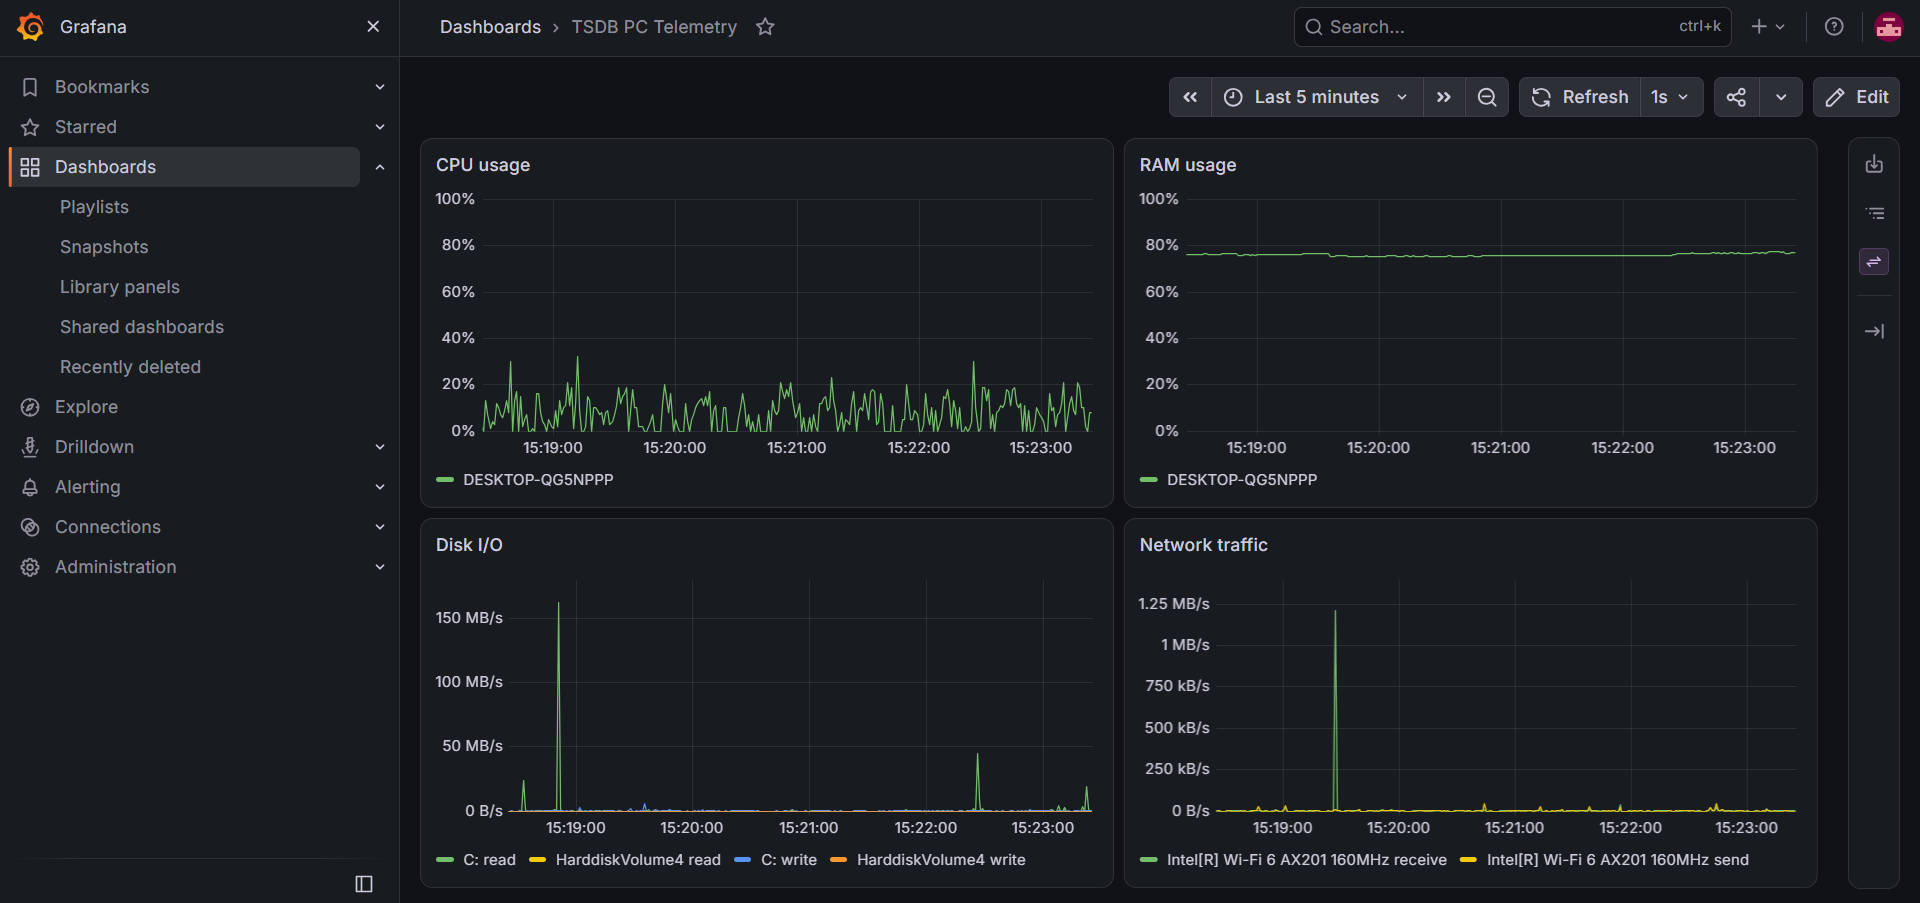
\includegraphics[width=\linewidth]{grafana_dashboard.png}
  \caption{Dashboard Grafany prezentujący rzeczywistą telemetrię komputera
  przechowywaną w TSDB.}
  \label{fig:grafana-dashboard}
\end{figure}

\begin{figure}[!htbp]
  \centering
  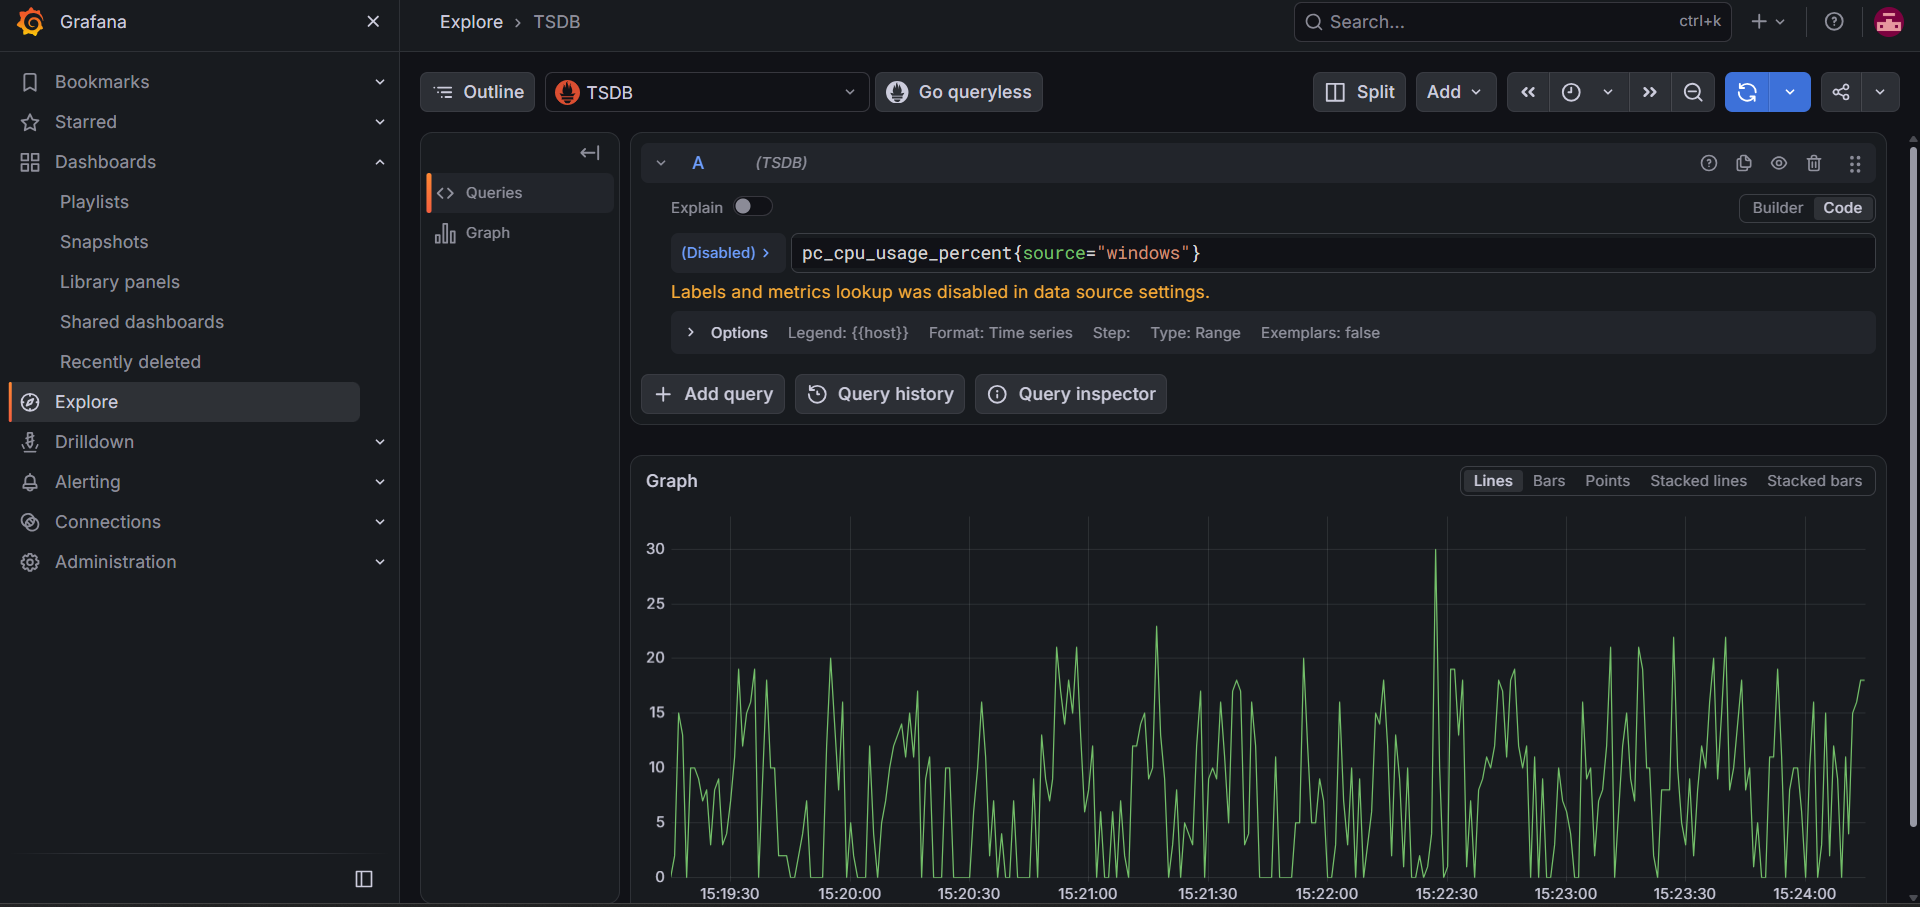
\includegraphics[width=\linewidth]{grafana_explore.png}
  \caption{Widok Explore: zapytanie o obciążenie CPU i otrzymany szereg czasowy.}
  \label{fig:grafana-explore}
\end{figure}
\FloatBarrier

\section{Pozostałe prace i najbliższy etap}
Najbliższy etap obejmuje agregacje czasowe: \mbox{\code{avg_over_time}}, \mbox{\code{min_over_time}},
\mbox{\code{max_over_time}}, \mbox{\code{sum_over_time}} i \mbox{\code{count_over_time}},
wraz z testami granic okien czasowych. Następnie należy uzupełnić obsługę
próbek poza kolejnością, ograniczyć blokowanie podczas operacji dyskowych
oraz przeprowadzić testy awarii i pomiary wydajności.
Retencja i kompaktowanie segmentów nie są zaimplementowane,
więc długotrwały zbiór telemetrii zwiększa zajętość dysku.

\end{document}
